\documentclass[titlepage]{article}
\usepackage[noerroretextools]{biblatex}
\usepackage{amsmath, amsthm, amsfonts}
\usepackage[capitalise]{cleveref}
\usepackage{bbm}
\usepackage{mathtools}
\usepackage{proba}
\usepackage{autonum}
\usepackage{enumerate}
\usepackage{sepfootnotes}
\usepackage{graphicx}
\usepackage{geometry}
\usepackage[labelfont=bf]{caption}
\usepackage{subcaption}
\usepackage{epstopdf}
\usepackage{pdflscape}
\usepackage{vub}
\usepackage{afterpage}
\usepackage[T1]{fontenc}
\usepackage{esint}

\addbibresource{bibliography.bib}
\graphicspath{{../plots/}}
\epstopdfsetup{outdir=../plots/}

\theoremstyle{plain}
\newtheorem{theorem}{Theorem}[section]
\newtheorem{lemma}{Lemma}[section]
\theoremstyle{definition}
\newtheorem{definition}{Definition}[section]

\newtheorem{proofpart}{Step}
\makeatletter
\@addtoreset{proofpart}{theorem}
\makeatother

\renewcommand\qedsymbol{QED}

\makeatletter
\newcommand{\itemref}[1]{%
  \begingroup % locally disable \perh@ps
  (\let\perh@ps\@gobble\ref{#1})%
  \endgroup
}
\makeatother

\DeclareRobustCommand{\cprobX}[3][{\mathbb{P}}]{\ensuremath{ {#1}\left( {#2} \mid {#3}\right)}}
\DeclareRobustCommand{\probX}[2][{\mathbb{P}}]{\ensuremath{ {#1}\left( {#2} \right)}}

\author{Othman El Hammouchi}
\title{L\'evy processes and their applications}
\subtitle{Exam assignment}
\faculty{Sciences and Bio-Engineering Sciences}

\sepfootnotecontent{fn:local-martingale}{For completeness, a stochastic process $\{ X_t \}$ is called a local martingale if there exists a sequence of stopping times $\{\tau_n \mid n \geq 1 \}$, almost surely increasing to infinity, such that the stopped process $X_{t \wedge \tau_n}$ is a martingale for every $n \geq 1$.}

\sepfootnotecontent{fn:kendall}{In queuing theory, it is standard to identify models using Kendall's notation, where the first letter identifies the distribution of the inter-arrival times, the second that of the service times, and the final entry gives the number of servers. An M/G/1 queue therefore has a single server, exponentially distributed (`Markovian') inter-arrival times, and its service times follow a general distribution.}

\sepfootnotecontent{fn:indicator}{In a slight abuse of notation, we will take $\mathbbm{1}_{ \{ W_t > 0 \} }$ to mean $\omega \mapsto \mathbbm{1}_{ \{ t \geq 0 \mid W_t(\omega) > 0 \} }$. This is consistent with \cite{kyprianou} and avoids the uglier alternative of $\mathbbm{1}_{\{ W_{\cdot} > 0 \}}$.}

\sepfootnotecontent{fn:laplace}{Or inverse transform, depending on the convention used.}

\begin{document}

\maketitle

\section{Introduction} \label{sec:intro}

Classical queueing theory is concerned with the study of stochastic dynamical systems in which certain 'events' occur randomly in time and require a random amount of work (time) to process. Examples of this include passengers checking in at the airport, requests arriving at a server over the network, or failures of industrial equipment in a factory requiring the attention of an engineer. We denote the volume of incoming work and the processed workload at time $t$ by $\{ A_t \}$ and $\{ B_t \}$, respectively, while the backlog at time $0$ is given by $w$. A simple instance of such a model is the M/G/1 queue\sepfootnote{fn:kendall}, in which we have $B_t = t$ and
\begin{equation}
  A_t = \sum_{i = 1}^{N_t} \xi_{i} \,.
\end{equation}
Here, $N_t$ a Poisson process with rate $\lambda$, giving the number of arrivals, and $\xi_i$ are i.i.d.\ random variables whose common distribution $F$, referred to as the \emph{service distribution}, describes the workload associated with a single arrival. The work inflow is thus given by a compound Poisson process in this case. We assume that new arrivals can only increase the workload (customers will not go behind the counter to help out the clerk), so that the support of $F$ is contained in $(0, +\infty)$.

While many applications can be modelled in terms of random streams of incoming and processed work, it is not always possible to express these in terms of discrete events. Consider, for example, the reservoir of a hydroelectric power station in a region with strong fluctuations in the water level---the inflow here must clearly represented by a continuous process. Another example comes from the realm of network traffic analysis, where it has been shown under certain assumptions (sufficiently slow growth in the connection rate) that the aggregate traffic over a high number of users approaches an $\alpha$-stable L\'evy motion (details can be found in \cite{mikosch}).

When the classical framework is extended to allow $A_t$ to be any L\'evy process, the resulting models are called \emph{L\'evy-driven queues} (see \cite{debicki} for an overview). The class of \emph{general storage models} refers to L\'evy-driven queues in which $A_t$ is a \emph{subordinator}.

\begin{definition}
  A L\'evy process is called a \emph{subordinator} if its sample paths are $a.s.$ non-decreasing.
\end{definition}

In this investigation, we will study how general storage models can be defined in terms of a so-called regulator, which will allow us to specify the workload process as a functional of the L\'evy input, and consider the distribution of the total idle time of the system. Our scope will be limited to the special case where $\{ A_t \}$ is of \emph{bounded variation}.

\begin{definition} \label{def:bounded-var}
  The total variation of a function $f: \mathbb{R}^+ \rightarrow \mathbb{R}$ over an interval $[a, b] \subset \mathbb{R}^+$ is defined as
  \begin{equation}
    V(f, [a, b]) \coloneqq \underset{{\pi \in \mathcal{P}}}{\mathrm{sup}} \sum_{i = 1}^{n - 1} \vert f(t_{i + 1}) - f(t_i) \vert \,,
  \end{equation}
  where the supremum runs over all partitions of the interval $[a, b]$. A stochastic process $\{ X_t \}$ is said to be of bounded variation if the total variation of its sample paths is finite over the interval $[0, t]$ for every $t > 0$.
\end{definition}

\section{Workload} \label{sec:workload}

Based on the definitions given in the previous section, it might seem tempting to define the \emph{workload} (the total amount of unprocessed work) of the system at any given time as
\begin{equation} \label{eq:work}
  D_t \coloneqq w + A_t - B_t = w + \sum_{i = 1}^{N_t} \xi_{i} - t \,,
\end{equation}
which is clearly a L\'evy process. The problem with this approach, however, is that $D_t$ can become negative, which would lead to a nonsensical situation. We could resolve this difficulty by adding another process $L_t$ with right-continuous increasing sample paths to $D_t$ which compensates for its negative sections, so that the sum $W_t \coloneqq D_t + L_t$ would become nonnegative everywhere. It is not difficult to see that the process $L_t \coloneqq -(\underset{s \leq t}{\mathrm{inf}} D_s \wedge 0)$ fits this bill. Moreover, it satisfies
\begin{equation} \label{eq:work-integral}
  \int \mathbbm{1}_{\{ W_t > 0 \}} dL_t = 0 \,,
\end{equation}
provided the integral can be defined in some appropriate sense\sepfootnote{fn:indicator}. If we can show that the sample paths of $L_t$ are monotone nondecreasing and right-continuous, we could define this expression pointwise in the underlying probability space as a Lebesgue-Stieltjes integral, i.e.\
\begin{equation}
  \int \mathbbm{1}_{\{ W_t(\omega) > 0 \}} dL_t(\omega) \coloneqq \int \mathbbm{1}_{\{ W_t(\omega) > 0 \}} d\mu_{L_t(\omega)} \,,
\end{equation}
where $\mu_{L_t(\omega)}$ is the Lebesgue-Stieltjes measure associated with $t \to L_t(\omega)$. Monotonicity follows from the monotonicity of the running infimum and the mapping $y \mapsto -(y \wedge 0)$. In order to demonstrate the second property, we will require the following lemma.

\begin{lemma} \label{lemma:running-inf-rc}
  Let $f: [0, +\infty) \rightarrow \mathbb{R}$ be a right-continuous function. Then the mapping
  \begin{equation}
    g(t) \coloneqq \mathrm{inf}_{s \leq t} f(s)
  \end{equation}
  will again be right-continuous.
\end{lemma}
\begin{proof}
  Let $t_n \downarrow t$ be a decreasing sequence in $\mathbb{R}$. We need to show that $g(t_n) \to g(t)$. As the value of the infimum on smaller sets can only increase, it follows that the sequence $g(t_n)$ is monotone. Seeking the contradiction, suppose that there exists an $\epsilon > 0$ such that $g(t_n) < g(t) - \epsilon$ for all $n \geq 1$. By the definition of the infimum, we can then find $s_n \leq t_n$ such that
  \begin{equation} \label{eq:cadlag-lemma-sn}
    f(s_n) < g(t) - \epsilon \leq f(t) - \epsilon \,, \quad n \geq 1 \,.
  \end{equation}
  Furthermore, it must be the case that $s_n > t$, otherwise we would have
  \begin{equation}
    f(s_n) \geq g(s_n) \geq g(t) \,
  \end{equation}
  which contradicts \cref{eq:cadlag-lemma-sn}. Hence, $t_n \leq s_n \leq t$, and the squeeze theorem from analysis gives us $s_n \to t$. By right-continuity of $f$, it follows that $f(s_n) \to f(t)$. However, \cref{eq:cadlag-lemma-sn} implies that $f(t) - f(s_n) > \epsilon$ for all $n$, hence we have a contradiction.
\end{proof}

As the mapping $y \to -(y \wedge 0)$ is continuous, it follows from \cref{lemma:running-inf-rc} that the composition $-(\mathrm{inf}_{s \leq t} f(s) \wedge 0)$ for a right-continuous mapping $f$ will again be right-continuous. In particular, by applying this pointwise to the sample paths of $\{ D_t \}$, we obtain that $t \mapsto L_t$ is a.s.\ c\`adl\`ag.

Any process which leads to a nonnegative result when added to $D_t$ is referred to as a \emph{regulator} for it; the sum $W_t$ is called the \emph{reflection} of $D_t$ at $0$. Because the compensation provided by a regulator is only required when $W_t = 0$, such a process can always be chosen to satisfy \cref{eq:work-integral}. In fact, it turns out that \cref{eq:work-integral} is enough to determine it uniquely.

\begin{theorem} \label{thm:regulator}
  Let $L_t$ be any stochastic process with increasing right-continuous sample paths such that
  \begin{enumerate}[(i)]
    \item $W_t = D_t + L_t \geq 0$ \label{cond:regulator-i}
    \item $\int \mathbbm{1}_{\{ W_t > 0 \}} dL_t = 0$ \,. \label{cond:regulator-ii}
  \end{enumerate}
  Then we have
  \begin{equation} \label{eq:reflection}
    L_t = -(\underset{s \leq t}{\mathrm{inf}} D_s \wedge 0) \,.
  \end{equation}
\end{theorem}

To prove \cref{thm:regulator}, we still need one further result from the theory of stochastic integration, proofs of which can be found in any standard textbook (see for example \cite[Theorem 3.17]{liptser}). Recall that a stochastic process $\{ X_t \}$ is called a \emph{semimartingale} if its paths are c\`adl\`ag and it admits a representation of the form
\begin{equation}
  X_t = M_t + A_t \,
\end{equation}
with $\{ M_t \}$ a local martingale\sepfootnote{fn:local-martingale}, $\{ A_t \}$ a process whose sample paths have bounded variation, and $M_0 = A_0 = 0$ a.s.

\begin{theorem}[Integration by parts] \label{thm:int-by-parts}
  If $\{ X_t \}$ and $\{ Y_t \}$ are semimartingales, then
  \begin{equation}
    X_t Y_t = X_0 Y_0 + \int_0^t X_{s-} d Y_s + \int_0^t Y_{s-} d X_s + [X, Y]_t \,.
  \end{equation}
\end{theorem}

The following proof is based on \cite[Proposition 2.3]{andersen}.

\begin{proof}[Proof of \cref{thm:regulator}]
  Writing $L^*_t  = -(\underset{s \leq t}{\mathrm{inf}} D_s \wedge 0)$, we begin by showing that this process satisfies \itemref{cond:regulator-i} and \itemref{cond:regulator-ii}. For the first property, notice that there are two possibilities: either $L^*_t = -\underset{s \leq t}{\mathrm{inf}} D_s$, in which case
  \begin{equation}
    W^*_t \coloneqq D_t + L^*_t = D_t - \underset{s \leq t}{\mathrm{inf}} D_s \geq 0 \,,
  \end{equation}
  or $L^*_t = 0$, implying that $D_t \geq \underset{s \leq t}{\mathrm{inf}} D_s \geq 0$ and hence $W^*_t = D_t \geq 0$. To see \itemref{cond:regulator-ii}, it suffices to observe that
  \begin{equation}
    \{ W^*_t = 0 \} = \{ D_t = (\underset{s \leq t}{\mathrm{inf}} D_s \wedge 0) \} = \{ t \in \mathrm{supp}(\mu_{L_t}) \} \,.
  \end{equation}

  To prove the uniqueness, we define
  \begin{equation}
    S_t \coloneqq L_t - L^*_t
  \end{equation}
  and demonstrate that this process vanishes everywhere. We have already shown that the sample paths of $L^*_t$ are increasing, and this holds for those of $L_t$ as well by assumption; the sample paths of both $L_t$ and $L^*_t$ are therefore of bounded variation. To see this, observe in \cref{def:bounded-var} that if $f$ is increasing, then $\sum_{i = 1}^{n - 1} \vert f(t_{i + 1}) - f(t_i) \vert = \sum_{i = 1}^{n - 1} (f(t_{i + 1}) - f(t_i)) = f(b) - f(a)$ for every $\pi$, so that $V(f, [a, b]) = f(b) - f(a)$ is finite. The result is obtained analogously for the case where $f$ is decreasing, and applying this to the sample paths of $L_t$ and $L^*_t$ yields the desired result.

  Consequently, $L_t$ and $L^*_t$ are semimartingales with $M_t \equiv 0$, hence the same is true of $S_t$ and we can apply \cref{thm:int-by-parts} to obtain
  \begin{align}
    S_t^2 & = 2 \int_0^t S_u dS_u + \sum_{u \leq t} (\Delta S_u)^2                                                    \\
          & =2 \int_0^t \{ L_u - L^*_u \} dL_u + 2 \int_0^t \{ L_u - L^*_u \} dL^*_u + \sum_{u \leq t} (\Delta S_u)^2 \\
          & =2 \int_0^t \{ W_u - W^*_u \} dL_u + 2 \int_0^t \{ W_u - W^*_u \} dL^*_u + \sum_{u \leq t} (\Delta S_u)^2 \\
          & =-2 \int_0^t W^*_u dL_u + 2 \int_0^t W_u dL^*_u + \sum_{u \leq t} (\Delta S_u)^2                          \\
          & \leq 0 \,
  \end{align}
  where we used the well-known fact that $[S, S]_t = \langle S \rangle_t = \sum_{u \leq t} (\Delta S_u)^2$ with $\Delta S_u \coloneqq S_u - S_{u-}$ the jump at $u$. The finally inequality follows from the nonnegativity of $W_t$ and $W^*_t$. In conclusion, we have that $S_t^2 \leq 0$, which is only possible if $L_t = L^*_t$.
\end{proof}

It's worth pausing a moment here to contemplate the meaning of \cref{eq:reflection}. At time $t = 0$, the counter opens and starts working on the backlog $w$ from the previous day. If the first arrival $T_1$ occurs before $w$, then $D_t$ will increase before it reaches $0$ and thus no intervention is needed from $L_t$. However, if $T_1$ takes place after $w$, then the clerk will have to wait idly for a while on the first customer and $D_t = w + \sum_{i = 1}^{N_t} \xi_i - t = w - t$ will become negative during this period. Hence, a compensation $L_t = -\underset{s \leq t}{\mathrm{inf}} D_s = t - w$ will need to be added in order to ensure that the workload remains $0$. At time $T_1$, the first customer comes to the counter and will require a processing time of $\xi_1 \sim F$ to complete his business. This causes $D_t$ to increase, meaning that $L_t$ will remain equal to $T_1 - w$ for a certain period of time. The same logic can be applied at subsequent arrival times $T_2, T_3, \dots$. The end result will be that \cref{eq:work} is used to describe the workload on $\{ W_t > 0 \}$, interspersed with exponentially distributed periods where $W_t = 0$. Example paths for $\{ X_t \}$ and $\{ W_t \}$ are shown in \cref{fig:example-paths}

\afterpage{
  \begin{landscape}
    \begin{figure}
      \centering
      \begin{subfigure}{0.45\linewidth}
        \centering
        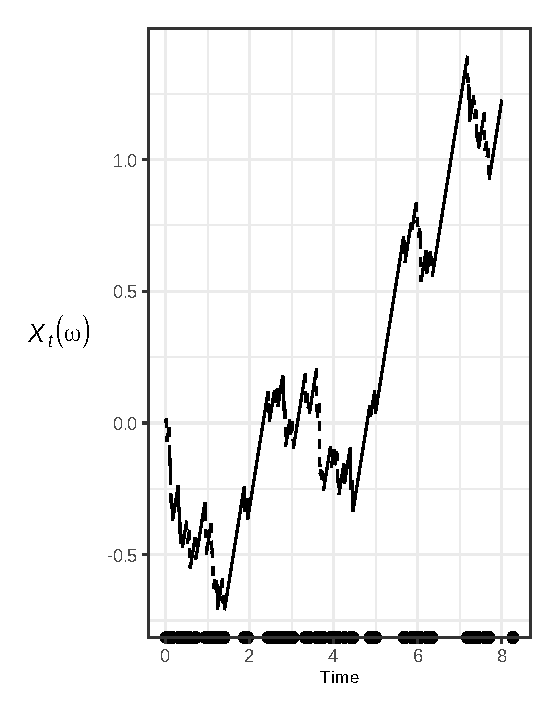
\includegraphics{input}
        \caption{Input}
      \end{subfigure}
      \begin{subfigure}{0.45\linewidth}
        \centering
        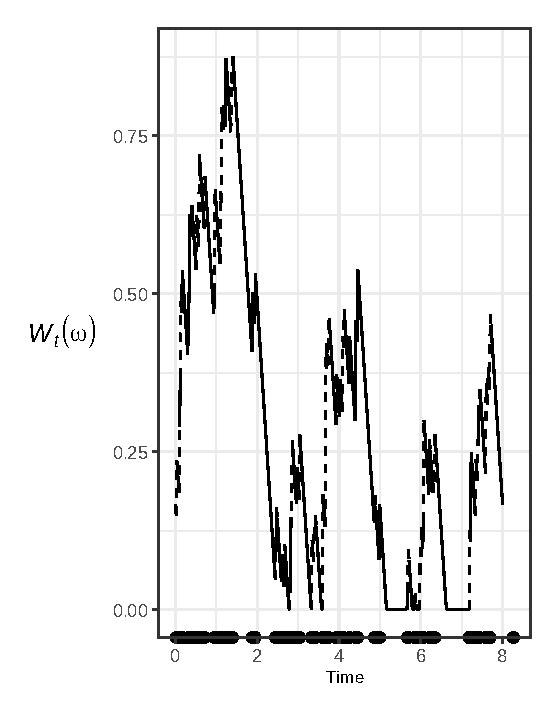
\includegraphics{workload}
        \caption{Workload}
      \end{subfigure}
      \caption{Example paths for the M/G/1 queue with $F \sim \Gamma$. The points on the x-axis represent arrival times.}
      \label{fig:example-paths}
    \end{figure}
  \end{landscape}
}

Finally, we remark that by writing $D_t = w - X_t$, it becomes possible to express $W_t$ as a function of an input process with negative jumps:
\begin{multline}
  W_t = D_t + L_t = -(\underset{s \leq t}{\mathrm{inf}} \{ w - X_s \} \wedge 0) + w - X_t = (\underset{s \leq t}{\mathrm{sup}} \{ X_s - w \} \vee 0) + w - X_t \\
  = (\overline{X}_t - w \vee 0) + w - X_t = (\overline{X}_t \vee w) - w + w - X_t = (\overline{X}_t \vee w) - X_t \,,
\end{multline}
where we defined $\overline{X}_t \coloneqq \underset{s \leq t}{\mathrm{sup}} X_s$. This representation will be useful in the following section.

\section{Idle time} \label{sec:idle-time}

A quantity of particular interest to us in the study of general storage models is the distribution of the total amount of time that the system is not processing any work, known as the \emph{idle time}. It serves as a measure of the efficiency of the system. If a processor in a parallel computation is spending a long time in spinlock, for example, this might point to a flaw in the program design or hardware configuration.

\begin{definition}
  The idle time of a general storage model is the integral
  \begin{equation}
    I \coloneqq \int_{(0, +\infty)} \mathbbm{1}_{\{ W_t = 0 \}} dt \,.
  \end{equation}
\end{definition}

Our aim is to derive the distribution of this quantity. We will first do this for the M/G/1 queue, allowing us to build some necessary tools and intuition, before moving on to the general case.

\begin{theorem} \label{thm:pois-idle-time}
  Let $\{ W_t \}$ be the workload process of an $M/G/1$ queue with arrival rate $\lambda$ and service distribution $F$ satisfying $\EX[\mathbb{E}_F]{X} = \mu$, and consider the function
  \begin{equation} \label{eq:psi-func}
    \psi(\theta) \coloneqq \theta - \lambda \int_{(0, +\infty)} \left( 1 - e^{-\theta x} \right) F(dx)  \,,
  \end{equation}
  defined for $\theta \geq 0$. Then the following hold:
  \begin{enumerate}[(i)]
    \item \label{pois_idle_time-i}
          If $\mu \lambda \leq 1$, then $I = +\infty$ a.s.
    \item \label{pois_idle_time-ii}
          If $\mu \lambda > 1$ and $\theta^*$ is the largest root of $\psi$, then
          \begin{equation}
            \prob_I = (1 - e^{-\theta^* w}) \delta_0 + \theta^* e^{-\theta^*{(w + x)}} \mathrm{Leb}
          \end{equation}
          where $\delta_0$ denotes the Dirac measure at $0$ and $\mathrm{Leb}$ is the Lebesgue measure.
  \end{enumerate}
\end{theorem}

To prove \cref{thm:pois-idle-time}, we require the following results from Sato's book (see \cite[Theorem 36.5 and Theorem 36.7]{sato}).

\begin{theorem}[Strong law of large numbers for Lévy processes] \label{thm:lln-levy}
  If $\{ X_t \}$ is a L\'evy process with $\EX{\vert X_1 \vert} < +\infty$ and $\EX{X_1} = c$ for some $c \in \mathbb{R}$, then
  \begin{equation}
    \lim_{t \to +\infty} \frac{X_t}{t} = c \quad \mathrm{a.s.}
  \end{equation}
\end{theorem}

Note that this implies $\lim_{t \to +\infty} X_t = +\infty$ if $c > 0$.

\begin{theorem} \label{thm:recurrent}
  Let $\{ X_t \}$ be a L\'evy process on $\mathbb{R}$. If $\EX{\vert X_1 \vert} < +\infty$ and $\EX{X_1} = 0$, then
  \begin{equation}
    \limsup_{t \to +\infty} X_t = +\infty \quad \mathrm{and} \quad \liminf_{t \to +\infty} X_t = -\infty \quad \mathrm{a.s.}
  \end{equation}
\end{theorem}

We will also need the following well-known theorem, a proof of which can be found, for example, in \cite[Theorem 3.2 and Corollary 3.6]{revuz}.

\begin{theorem}[Optional sampling] \label{thm:opt-samp}
  Let $X_t$ be a right-continuous martingale and consider a stopping time $\tau: \Omega \rightarrow [0, +\infty]$. Then the \emph{stopped process}
  \begin{equation}
    X^\tau_t \coloneqq X_{\tau \wedge t}
  \end{equation}
  will again be a martingale.
\end{theorem}

\begin{proof}[Proof of \cref{thm:pois-idle-time}]
  \begin{proofpart}
    Observe that the integral in \cref{eq:psi-func} is finite because $\vert e^{-\theta x} \mathbbm{1}_{(0, +\infty)} \vert \leq 1$. We begin by showing that $\psi$ is the natural logarithm of the Laplace transform\sepfootnote{fn:laplace} of $X_1$ on $\mathbb{R}^+$. For $\theta \geq 0$ we have
    \begin{align}
      \EX{e^{\theta X_t}} & = \EX{e^{\theta (t - \sum_{i = 1}^{N_t} \xi_i)}}                                                                                                               \\
                          & = \sum_{n = 0}^\infty \frac{(\lambda t)^n}{n!} e^{-\lambda t} \EX{e^{\theta (t - \sum_{i = 1}^n \xi_i)}}                                                       \\
                          & = e^{-\lambda t} \sum_{n = 0}^\infty \frac{(\lambda t)^n}{n!}  \int_{(0, +\infty)} e^{\theta t} \prod_{i = 1}^n e^{-\theta x_i} \, F(dx_1, \dots, dx_n)        \\
                          & = e^{-\lambda t} \sum_{n = 0}^\infty \frac{(\lambda t)^n}{n!} e^{\theta t} \idotsint_{(0, +\infty)^n} \prod_{i = 1}^n e^{-\theta x_i} \, F(dx_1) \dots F(dx_n) \\
                          & = e^{(\theta - \lambda) t} \sum_{n = 0}^\infty \frac{(\lambda t)^n}{n!} \left( \int_{(0, +\infty)} e^{-\theta x} \, F(dx) \right)^n                            \\
                          & = e^{(\theta - \lambda) t} e^{\lambda t \int_{(0, +\infty)} e^{-\theta x} \, F(dx)} \,.
    \end{align}
    Hence, it follows that
    \begin{align}
      \log{(\EX{e^{\theta X_t}})} & = \theta t - \lambda t \left( 1 -  \int_{(0, +\infty)} e^{-\theta x} F(dx) \right) \\
                                  & = \theta t - \lambda t \int_{(0, +\infty)} (1 - e^{-\theta x}) F(dx) \,,
    \end{align}
    and the desired result is obtained by substituting $t = 1$. Note moreover that
    \begin{equation} \label{eq:laplace-time-scaling}
      \EX{e^{\theta X_t}} = e^{t \psi(\theta)} = \EX{e^{\theta X_1}}^t \,.
    \end{equation}

    From the analyticity of the Laplace transform on its convergence region, it follows that $\psi$ is continuous and infinitely differentiable. This function is known as the \emph{Laplace exponent} of $X_1$, and $e^{\psi(\theta)}$ can be viewed as a one-sided moment-generating function. Indeed, for any $\theta > 0$, we can apply the dominated convergence theorem (using the fact that $X_t \leq t$) to obtain
    \begin{align}
      \psi^{(n)}(\theta) = \EX{X_1^n e^{\theta X_1}} \,,
    \end{align}
    from which it follows, by taking one-sided limits and using the DCT a second time, that
    \begin{equation} \label{eq:first-moment}
      \psi^{(n)}(0+) = \lim_{\theta \underset{>}{\to} 0} \psi^{(n)}(\theta) = \EX{X_1^n} \,,
    \end{equation}
    and
    \begin{equation}
      \psi''(\theta) = \lambda \int_{(0, +\infty)} x^2 e^{-\theta x} \, F(dx) \geq 0 \,.
    \end{equation}
    In particular, we see that
    \begin{equation} \label{eq:right-deriv}
      \EX{X_1} = \psi'(0+) = \lim_{\theta \underset{>}{\to} 0} \left( 1 - \lambda \int_{(0, +\infty)} x e^{-\theta x} F(dx) \right) = 1 - \lambda \mu \,.
    \end{equation}
    Moreover, for any sequence $(\theta_n)_n \subset (0, +\infty)$ with $\theta_n \downarrow 0$, we have
    \begin{equation}
      1 = \EX{\lim_{n \to \infty} e^{\theta_n X_1}} = \lim_{n \to \infty} \EX{e^{\theta_n X_1}} = \lim_{n \to \infty} e^{\psi(\theta_n)} \,
    \end{equation}
    (the interchange of limit and expectation again being justified by the DCT), from which it follows that $\psi(\theta_n) \xrightarrow{n \to \infty} 0$ and hence $\lim_{\theta \underset{>}{\to} 0} \psi(\theta) = 0$. From $e^{\psi(\theta)} \geq \EX{e^{\theta X_1} \mathbbm{1}_{\{ X_1 > 0\}}} \xrightarrow{\theta \to \infty} +\infty$, we also deduce that $\lim_{\theta \to \infty} \psi(\theta) = \infty$. Taking these properties together, we conclude that $\psi$ is a convex function going from $0$ to $\infty$, and that there are consequently two possibilities for its intermediate behaviour: either $\psi'(0+) \geq 0$, in which case $\psi$ does not cross the x-axis a second time, or $\psi'(0+) < 0$ and $\psi$ has an additional root in $(0, +\infty)$. These correspond to the cases $\lambda \mu \leq 1$ and $\lambda \mu > 1$ distinguished in the statement of the theorem.
  \end{proofpart}

  \begin{proofpart}
    Next, consider the stochastic process
    \begin{equation}
      Y_t \coloneqq \{ e^{\theta X_t - \psi(\theta) t} \mid t \geq 0 \} \,,
    \end{equation}
    for any $\theta > 0$. Using the previous results, we will show that this is a martingale with respect to the filtration
    \begin{equation}
      \mathfrak{F} = \left( \mathcal{F}_t \right)_{t \geq 0} \coloneqq \left( \sigma \{X_u \mid u \leq t\} \right)_{t \geq 0} \,.
    \end{equation}
    Because the mapping $x \mapsto \exp{(\theta x - \psi(\theta) t)}$ is continuous, it follows immediately that $Y_t$ is adapted. Moreover, as
    \begin{equation}
      \EX{\vert Y_t \vert} = e^{-\psi(\theta) t} \EX{e^{\theta X_t}} = 1 < \infty \,,
    \end{equation}
    we have $Y_t \in L^1(\Omega)$ for every $t \geq 0$. Finally, the martingale property follows by using the stationary independent increments property of $X_t$ to obtain, for $t > s$,
    \begin{equation} \label{eq:martingale-property}
      \begin{aligned}
        \cEX{Y_t}{\mathcal{F}_s} & = e^{\theta X_s - \psi(\theta) s} \cEX{e^{\theta (X_t - X_s) - \psi(\theta) (t - s)}}{\mathcal{F}_s} \\
                                & = e^{\theta X_s - \psi(\theta) s} \EX{e^{\theta (X_t - X_s) - \psi(\theta) (t - s)}}                 \\
                                & = e^{\theta X_s - \psi(\theta) s} \EX{e^{\theta X_{t - s}}} e^{-\psi(\theta) (t - s)}                \\
                                & = e^{\theta X_s - \psi(\theta) s} = Y_s \,.
      \end{aligned}
    \end{equation}
  \end{proofpart}

  \begin{proofpart}
    Now let $\tau^+_x$ be the first time after $0$ that the process $X_t$ exceeds the threshold $x$, i.e.\
    \begin{equation} \label{eq:first-passage}
      \tau^+_x \coloneqq \mathrm{inf}\{ t \geq 0 \mid X_t > x \} \,.
    \end{equation}
    This is a stopping time; to see this, observe that
    \begin{equation}
      \{ \tau_x^+ < t \} = \bigcup_{0 \leq s < t} \{ X_s > x \} \,,
    \end{equation}
    hence $\omega \in \{ \tau_x^+ < t \} \iff \exists s < t : X_s > x$. Consequently, by choosing $(s_n)_n \subset \mathbb{Q}$ such that $s_n \downarrow s$ and using the right-continuity of $\{ X_t \}$, we obtain that $X_{s_k} > x$ for $k$ sufficiently large, whence it follows that
    \begin{equation}
      \{ \tau_x^+ < t \} = \bigcup_{s \in \mathbb{Q} \cap [0, t)} \ \{ X_s > x \} \in \mathcal{F}_t \,.
    \end{equation}

    If $\lambda \mu \leq 1$, it follows from \cref{eq:right-deriv,eq:first-moment} that $\EX{X_1} \geq 0$; hence, either $\EX{X_1} > 1$ and we can apply \cref{thm:lln-levy} to conclude that $\lim_{t \to +\infty} X_t = +\infty$ a.s., or $\EX{X_1} = 0$ and by \cref{thm:recurrent}, $\limsup_{t \to +\infty} X_t = +\infty$ a.s. In both cases we can conclude that $\overline{X}_\infty = +\infty$ a.s. On the other hand, if $\lambda \mu > 1$, then $\psi$ has an additional root $\theta^* > 0$, and we can apply \cref{thm:opt-samp} to $Y_t$ to obtain
    \begin{equation} \label{eq:opt-sample-res}
      1 = \EX{Y_{t \wedge \tau^+_x}} = \EX{e^{\theta^* X_{t \wedge \tau^+_x} - \psi(\theta) (t \wedge \tau_x^+)}} \,.
    \end{equation}
    On the event $\{ \tau_x^+ = +\infty \}$, we have $X_{t \wedge \tau_x^+} = X_t \leq x$ and hence $Y_{t \wedge \tau_x^+} \xrightarrow{t \to +\infty} 0$. Taking the limit as $t \to +\infty$ of both sides in \cref{eq:opt-sample-res} therefore yields
    \begin{equation}
      1 = \EX{e^{\theta^* X_{\tau^+_x}} \mathbbm{1}_{\{\tau^+_x < \infty \}}} = e^{\theta^* x} \probX{\tau^+_x < \infty} = e^{\theta^* x} \probX{\overline{X}_\infty > x} \,,
    \end{equation}
    where $X_{\tau^+_x} = x$ follows from the fact that $\{ X_t \}$ has no negative jumps, and $\overline{X}_\infty(\omega) \coloneqq \lim_{t \to +\infty} \overline{X}_t(\omega)$. Note that this last limit is guaranteed to exist for all $\omega \in \Omega$ because the paths of $\{ \overline{X}_t \}$ are non-decreasing (allowing for values of $+\infty$). Hence, $\probX{\overline{X}_\infty \leq x} = 1 - e^{-\theta^* x}$, and we see that $\overline{X}_\infty$ follows an exponential distribution with parameter $\theta^*$.
  \end{proofpart}

  \begin{proofpart}
    From the definition of $\{ W_t \}$ we immediately get that $\{ W_t = 0 \} = \{ \overline{X}_t = X_t \} \cap {\{ \overline{X_t} > w \}}$. If we now define
    \begin{equation}
      T_1 \coloneqq \mathrm{inf} \{ t > 0 \mid X_{t-} \neq X_t \}
    \end{equation}
    and
    \begin{equation}
      T_k \coloneqq \mathrm{inf} \{ t > T_{k - 1} \mid X_t > X_{T_{k - 1}} \}
    \end{equation}
    for $k \geq 2$, then, on the event $\{ \overline{X}_t \neq X_t \} \cap {\{ \overline{X_t} > w \}}$, we have
    \begin{equation}
      \overline{X}_s = \sum_{k = 1}^\infty \overline{X}_{T_k} \mathbbm{1}_{[T_k, T_{k + 1})}
    \end{equation}
    and $\overline{X}_t = X_t = t + c_k$ on $\{ \overline{X}_t = X_t \} \cap {\{ \overline{X_t} > w \}}$, where $c_k$ is a real constant depending on the interval $[T_k, T_{k + 1})$. Consequently, it follows that
    \begin{align}
      (\overline{X}_t - w) \vee 0 & = \int_0^t \mathbbm{1}_{{\{ \overline{X_u} > w \}} } d\overline{X}_u                                                                                                                                           \\
                                  & = \int_0^t \mathbbm{1}_{ \{ \overline{X}_u = X_u \} \cap {\{ \overline{X_u} > w \}} } d\overline{X}_u + \int_0^t \mathbbm{1}_{ \{ \overline{X}_u \neq X_u \} \cap {\{ \overline{X_u} > w \}} } d\overline{X}_u \\
                                  & = \int_0^t \mathbbm{1}_{ \{ \overline{X}_u = X_u \} \cap {\{ \overline{X_u} > w \}} } d\overline{X}_u                                                                                                          \\
                                  & = \int_0^t \mathbbm{1}_{ \{W_u = 0 \} } du \,,
    \end{align}
    where the existence of the first integral follows using the same arguments as in \cref{sec:workload}. Finally, we can apply the monotone convergence theorem (the version allowing $\infty$) to obtain
    \begin{equation}
      I = \int_0^\infty \mathbbm{1}_{\{ W_u = 0 \}} du = (\overline{X}_\infty - w) \vee 0 \,.
    \end{equation}
  \end{proofpart}

  \begin{proofpart}
    As we've established previously, $\lambda \mu \leq 1$ implies $\overline{X}_\infty = +\infty$ a.s., hence $I = +\infty$ a.s. If $\lambda \mu > 1$, then $\overline{X}_\infty \sim \mathrm{Exp}(\theta^*)$ and $\probX{\tau^+_w = \infty} = \probX{\overline{X}_\infty \leq w} = 1 - e^{-\theta^* w}$. Since $I = 0$ when $\overline{X}_\infty \leq w$, we thus obtain
    \begin{equation}
      \probX{\{ I \in B \} \cap \{ \tau^+_w = \infty \}} =
      \begin{cases}
        \probX{\tau^+_w = \infty} = 1 - e^{-\theta^* w} & \text{if} \ 0 \in B \\
        0                                               & \text{otherwise}
      \end{cases} \,,
    \end{equation}
    for any $B \in \mathcal{B}(\mathbb{R})$. Additionally, for $x \geq 0$, we also have
    \begin{align}
      \probX{\{ I > x \} \cap \{ \tau^+_w < \infty \}} & = \probX{\{ \overline{X}_\infty - w > x\} \cap \{ \overline{X}_\infty > w \}}                      \\
                                                       & = \cprobX{ \overline{X}_\infty > x + w }{\overline{X}_\infty > w } \probX{\overline{X}_\infty > w} \\
                                                       & = e^{-\theta^*{(x + w)}}                                                                           \\
                                                       & = \int_x^\infty \theta^* e^{-\theta^*{(y + w)}} \, dy
      \,.
    \end{align}
    Putting these two together, we conclude that
    \begin{equation}
      \prob_I = (1 - e^{-\theta^* w}) \delta_0 + \theta^* e^{-\theta^*{(w + x)}} \mathrm{Leb} \,,
    \end{equation}
    which proves (\ref{pois_idle_time-ii}).
  \end{proofpart}
\end{proof}

\afterpage{
  \begin{landscape}
    \begin{figure}
      \centering
      \begin{subfigure}{0.45\linewidth}
        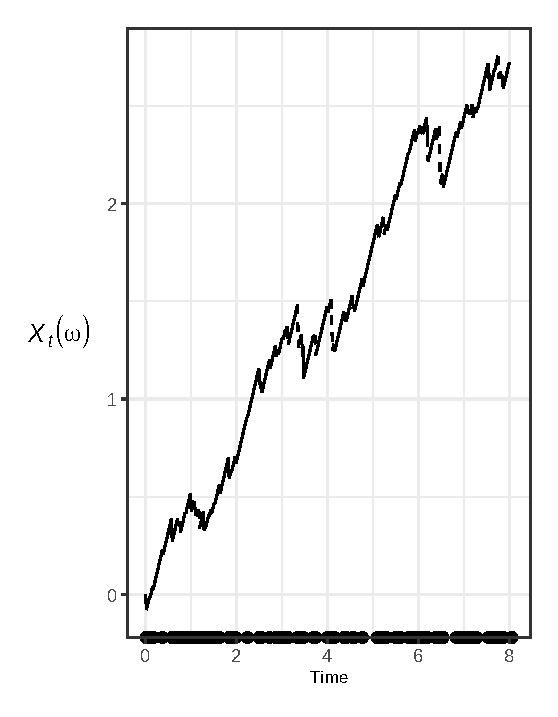
\includegraphics{input_leq_1}
        \caption{Input}
      \end{subfigure}
      \begin{subfigure}{0.45\linewidth}
        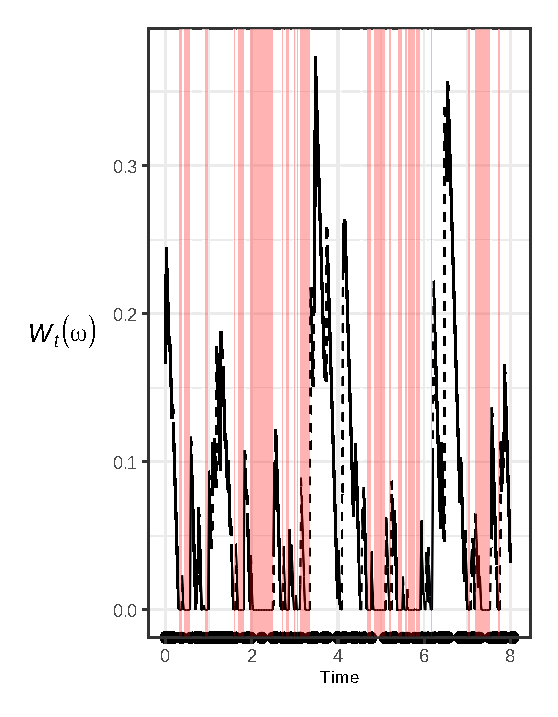
\includegraphics{workload_leq_1}
        \caption{Workload}
      \end{subfigure}
      \caption{Example paths for the M/G/1 queue with $\lambda \mu \leq 1$. The points on the x-axis represent arrival times, and the shaded regions are idle periods.}
      \label{fig:example-leq-1}
    \end{figure}
    \pagebreak
    \begin{figure}
      \centering
      \begin{subfigure}{0.45\linewidth}
        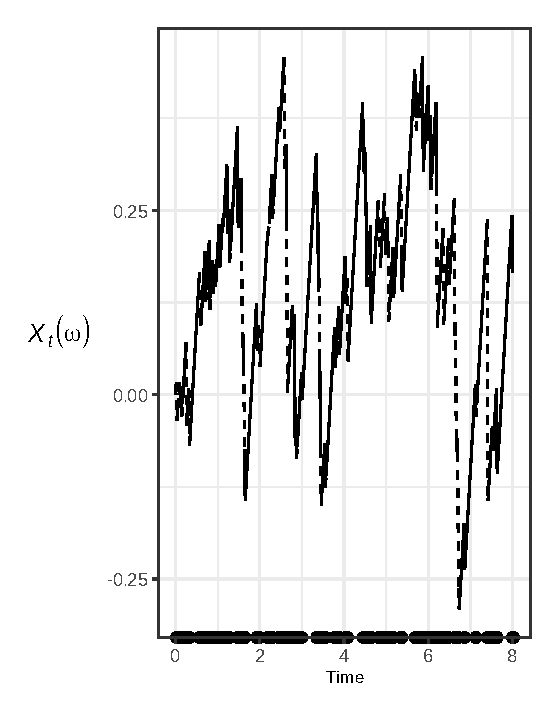
\includegraphics{input_ge_1}
        \caption{Input}
      \end{subfigure}
      \begin{subfigure}{0.45\linewidth}
        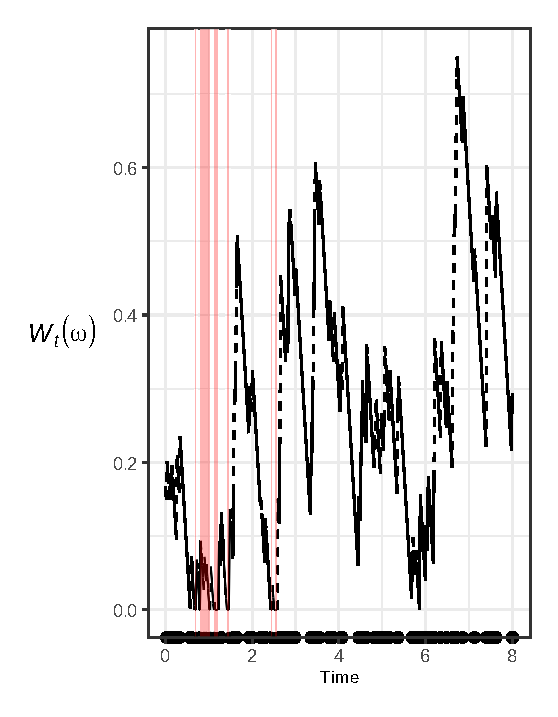
\includegraphics{workload_ge_1}
        \caption{Workload}
      \end{subfigure}
      \caption{Example paths for the M/G/1 queue with $\lambda \mu > 1$. The points on the x-axis represent arrival times, and the shaded regions are idle periods.}
      \label{fig:example-ge-1}
    \end{figure}
  \end{landscape}
}

The next two pages show example paths of $\{ X_t \}$ and $\{ W_t \}$ for both $\lambda \mu \leq 1$ and $\lambda \mu > 1$. As we can see, in the former case, idle periods persist as $t \to +\infty$. By contrast, when there is heavy traffic ($\lambda \mu > 1$), we observe less and less idle periods as time goes on, and they eventually die out completely.

The crucial part in the proof \cref{thm:pois-idle-time} was identifying the relationship between $I$ and $\overline{X}_\infty$, as the distribution of the latter could be analysed using martingale techniques and the Laplace exponent. We will employ a similar reasoning in the more general setting where $X_t = t - A_t$ with $\{ A_t \}$ a subordinator of bounded variation, hence we begin by showing that the Laplace transform on $\mathbb{R}^+$ is finite as well in this case.

\begin{lemma}
  $\EX{e^{\theta X_1}} < \infty$ for every $\theta \geq 0$
\end{lemma}

\begin{proof}
  For $\theta \geq 0$ fixed, let $\mathbf{e}_q$ be an exponentially distributed random variable with rate parameter $q$, independent from $\{ X_t \}$, and consider $\overline{X}_{\mathbf{e}_q}$. We will show that this random variable follows a $\mathrm{Exp}(\lambda)$ distribution for some $\lambda > 0$. To see this, observe that the first passage time process $\{ \tau^+_x \mid x \geq 0 \}$ is a subordinator, as its sample paths are generalised inverses of the sample paths of $\{ X_t \}$ (cfr.\ \cref{eq:first-passage}), which are nondecreasing and continuous (for a rigorous argument, see \cite[Chapter VII, Theorem 1]{bertoin}). Using the lack of memory property and the fact that the increments of $\{ t_x^+ \}$ are independent and stationary, we then obtain
  \begin{align}
    \probX{\overline{X}_{\mathbf{e}_q} > x + y} & = \probX{\tau_{x + y}^+ < \mathbf{e}_q}                                                                                   \\
                                                & = \cprobX{\tau_x^+ + (\tau_{x + y}^+ - \tau_x^+) < \mathbf{e}_q}{\tau_x^+ < \mathbf{e}_q} \probX{\tau_x^+ < \mathbf{e}_q} \\
                                                & = \probX{\tau_{x + y}^+ - \tau_x^+ < \mathbf{e}_q} \probX{\tau_x^+ < \mathbf{e}_q}                                        \\
                                                & = \probX{\tau_y^+ < \mathbf{e}_q} \probX{\tau_x^+ < \mathbf{e}_q}                                                         \\
                                                & =  \probX{\overline{X}_{\mathbf{e}_q} > x } \probX{\overline{X}_{\mathbf{e}_q} > y} \,,
  \end{align}
  hence memorylessness holds for $\overline{X}_{\mathbf{e}_q}$ as well, and this property uniquely defines the exponential distribution. In view of the fact that $\probX{\mathbf{e}_q < \varepsilon} = 1 - e^{-q \varepsilon} \xrightarrow{q \to +\infty} 1$ for every $\varepsilon > 0$, it follows that $\mathbf{e}_q \xrightarrow{\prob} 0$ as $q \to +\infty$. Using the continuity of the paths of $\{ \overline{X}_t \}$, we obtain $\overline{X}_{\mathbf{e}_q} \xrightarrow{\prob} \overline{X}_0 = X_0 = 0$, hence it follows that $\lambda \to \infty$. Thus, it is always possible to obtain $\lambda > \theta$ by choosing $q$ sufficiently large, and for such a $q$ we have
  \begin{equation}
    \int_0^\infty q e^{-q t} \EX{e^{\theta \overline{X}_t}} \, dt = \EX{e^{\theta \overline{X}_{\mathbf{e}_q}}} < +\infty \,
  \end{equation}
  where the finiteness follows from the fact that the moment-generating function of the exponential distribution has convergence region $(-\infty, \lambda)$. It follows that $\EX{e^{\theta X_t}} \leq \EX{e^{\theta \overline{X}_t}} < \infty$ for every $t \geq 0$, hence $\EX{e^{\theta X_1}} < +\infty$ as desired.
\end{proof}

It follows that the Lévy-Khintchine exponent has an analytic extension to the lower complex halfplane, yielding the expression
\begin{align} \label{eq:laplace-exponent}
  \psi(\theta) \coloneqq \log{\phi(-i \theta)} & = \gamma \theta + \frac{1}{2} A \theta^2 + \int_\mathbb{R} (e^{\theta x} - 1 - \theta x \mathbbm{1}_{\{ \vert x \vert < 1 \}}) \, \nu(dx)               \\
                                               & = \gamma \theta + \frac{1}{2} A \theta^2 + \int_{(-\infty, -1]} (e^{\theta x} - 1) \, \nu(dx) + \int_{(-1, 0)} (e^{\theta x} - 1 - \theta x) \, \nu(dx)
\end{align}
for the Laplace exponent. The second equality follows from the fact that
\begin{equation}
  \#\{ 0 < s \leq t \mid X_s - X_{s-} \in B \} = t \nu(B)
\end{equation}
for any $t \geq 0$ and $B \in \mathcal{B}(\mathbb{R})$ with $0 \notin B$, hence $\nu((0, +\infty)) = 0$ for a process with no positive jumps. The function $\psi$ satisfies the same properties as those described in the proof of \cref{thm:pois-idle-time}.

\begin{lemma}
  $\psi(\theta)$ is an infinitely differentiable, strictly convex convex function from $[0, \infty)$ to $\mathbb{R}$ with $\psi(0) = 0$ and $\lim_{\theta \to \infty} \psi(\theta) = \infty$.
\end{lemma}

\begin{proof}
  It immediately follows from the definition that $\psi(0) = 0$, and infinite differentiability is likewise a property of the Laplace transform. From $e^{\psi(\theta)} \geq \EX{e^{\theta X_1} \mathbbm{1}_{\{ X_1 > 0\}}} \xrightarrow{\theta \to \infty} +\infty$, we also deduce that $\lim_{\theta \to \infty} \psi(\theta) = \infty$. As for the convexity, observe that we have $\vert e^{\theta x} - 1 \vert \leq 2$ on $(-\infty, -1]$ and from Taylor's theorem
  \begin{equation}
    \vert e^{\theta x} - 1 - \theta x \vert \leq e^\theta x^2
  \end{equation}
  on $(-1, 0)$. Hence, starting from \cref{eq:laplace-exponent}, we can apply the dominated convergence theorem to differentiate under the integral sign, giving us
  \begin{equation}
    \psi''(\theta) = A + \int_{(-\infty, 0)} x^2 e^{\theta x} \, dx > 0
  \end{equation}
\end{proof}

If we now define the generalised right inverse of $\psi$ as
\begin{equation}
  \Phi(q) \coloneqq \mathrm{sup}\{ \theta \geq 0 \mid \psi(\theta) = q \} \,
\end{equation}
with $(\psi \circ \Phi)(q) = q$. There will again be two possibilities for $\Phi(0)$. If $\psi'(0+) > 0$, then $0$ is the unique root of $\psi$, and $\Phi(0) = 0$. On the other hand, if $\psi'(0+) < 0$, the function $\psi$ will have an additional root in $(0, +\infty)$, hence $\Phi(0) > 0$. These two regimes will determine two different possibilities for the distribution of the idle time, just as in \cref{thm:pois-idle-time}.

Before we can prove a generalisation of \cref{thm:pois-idle-time}, we still need one additional lemma.

\begin{theorem} \label{thm:inverse-laplace-exp}
  $\EX{e^{-q \tau_x^+} \mathbbm{1}_{\{ \tau_x^+ < +\infty \}}} = e^{-\Phi(q) x}$ for any $q \geq 0$.
\end{theorem}

The function $\Phi$ can thus be viewed as an `inverse Laplace exponent' of the subordinator $\{ \tau_x^+ \}$.

\begin{proof} 
  We will use martingale techniques similar to the proof of \cref{thm:pois-idle-time}. If we define the process
  \begin{equation}
    Y_t \coloneqq e^{\Phi(q) X_t - q t} \,
  \end{equation}
  then
  \begin{equation}
    \EX{\vert Y_t \vert} = e^{-q t} \EX{e^{\Phi(q) X_t}} = e^{-q t} e^{\psi(\Phi(q)) t} = 1 < +\infty
  \end{equation}
  Continuity of $y \mapsto e^{\Phi(q)y - q t}$ guarantees that $Y_t$ is adapted to the filtration generated by $\{ X_t \}$, and the martingale property follows from the independent stationary increments property in the same way as in \cref{eq:martingale-property}. Hence we can apply \cref{thm:opt-samp} with $\tau = \tau_x^+$ to obtain
  \begin{equation} \label{eq:stopped-martingale}
    \EX{Y_{t \wedge \tau_x^+}} = \EX{e^{\Phi(q) X_{t \wedge \tau_x^+} - q (t \wedge \tau_x^+)}} = 1 \,.
  \end{equation}

  On the event $\{ \tau_x^+ = +\infty \}$, we have $X_t \leq x$ for all $t \geq 0$ and hence
  \begin{equation}
    e^{\Phi(q) X_{t \wedge \tau_x^+} - q (t \wedge \tau_x^+)} = e^{\Phi(q) X_t - q t} \leq e^{\Phi(q) x - q t} \xrightarrow{t \to +\infty} 0 \,.
  \end{equation}
  Using the dominated convergence theorem, it therefore follows that $\EX{Y_{t \wedge \tau_x^+} \mathbbm{1}_{\{ \tau_x^+ = +\infty \}}} \to 0$ as $t \to +\infty$. Consequently, taking this same limit on both sides of \cref{eq:stopped-martingale} and using the fact that $X_{\tau_x^+} = x$ (because the process only has negative jumps), we obtain
  \begin{equation}
    \EX{e^{\Phi(q) x - q \tau_x^+}} = 1 \,,
  \end{equation}
  which proves the theorem.
\end{proof}

\begin{theorem} \label{thm:gen-idle-time}
  Defining the \emph{traffic intensity} as
  \begin{equation}
    \rho \coloneqq 1 - \psi'(0+) \,,
  \end{equation}
  we then have:
  \begin{enumerate}[(i)]
    \item $I = +\infty$ a.s. if $0 < \rho \leq 1$.
    \item The distribution of $I$ is given by
          \begin{equation}
            \prob_I = (1 - e^{-\Phi(0)w}) \delta_0 + \Phi(0) e^{-\Phi(0)(w + x)} \mathrm{Leb}
          \end{equation}
          if $\rho > 1$.
  \end{enumerate}
\end{theorem}

\begin{proof}
  In view of the fact that the sample paths of $\{ X_t \}$ have bounded variation, we can write
  \begin{align}
    \overline{X}_t & = \int_0^t d\overline{X}_s                                                                                                \\
                   & = \int_0^t \mathbbm{1}_{\{ \overline{X}_u = X_u \}} \, dX_u                                                               \\
                   & = \int_0^t \mathbbm{1}_{\{ \overline{X}_u = X_u \}} \, du - \int_0^t \mathbbm{1}_{\{ \overline{X}_u = X_u \}} \, dA_u \,.
  \end{align}
  Additionally, as the process only has negative jumps, it follows that $\Delta A_u = 0$ whenever $\overline{X}_u = X_u$, which implies
  \begin{equation}
    \int_0^t \mathbbm{1}_{\{ \overline{X}_u = X_u \}} dA_u \leq \int_0^t \mathbbm{1}_{\{ \Delta A_u = 0 \}} dA_u = 0 \,,
  \end{equation}
  and consequently
  \begin{equation}
    \overline{X}_t = \int_0^t \mathbbm{1}_{\{ \overline{X}_u = X_u \}} du \,.
  \end{equation}

  If $w = 0$, the monotone convergence theorem yields
  \begin{equation}
    \overline{X}_\infty = \int_0^\infty \mathbbm{1}_{\{ \overline{X}_u = X_u \}} du = \int_0^\infty \mathbbm{1}_{\{ W_u = 0 \}} du = I \,.
  \end{equation}
  To derive the distribution of $\overline{X}_\infty$, we again consider $\overline{X}_{\mathbf{e}_q}$ as defined previously. Using \cref{thm:inverse-laplace-exp}, we can then deduce that
  \begin{align}
    \probX{\overline{X}_{\mathbf{e}_q} > x} & = \EX{\mathbbm{1}_{\{\overline{X}_{\mathbf{e}_q} > x \}}} \\
                                            & = \EX{\mathbbm{1}_{\{ \tau_x^+ < \mathbf{e}_q \}}}        \\
                                            & = \EX{\int_{\tau_x^+}^\infty q e^{-qt} \, dt}             \\
                                            & = \EX{-(0 - e^{-q \tau_x^+})} = e^{-\Phi(q)x} \,,
  \end{align}
  i.e.\ $\overline{X}_{\mathbf{e}_q} \sim \mathrm{Exp}(\Phi(q))$. Additionally, because we have
  \begin{equation}
    \lim_{q \downarrow 0} \probX{\overline{X}_{\mathbf{e}_q} > x} = \probX{\lim_{q \downarrow 0} \overline{X}_{\mathbf{e}_1 / q} > x} = \probX{\overline{X}_\infty > x} \,,
  \end{equation}
  it follows that $\overline{X}_{\mathbf{e}_q} \xrightarrow{d} \overline{X}_\infty$ and $\overline{X}_\infty \sim \mathrm{Exp}(\Phi(0))$. For $0 < \rho \leq 1$, we will have $\Phi(0) = 0$ and hence $I \overset{d}{=} \overline{X}_\infty \sim \mathrm{Exp}(0)$, which we interpret to mean $\overline{X}_\infty = +\infty$ a.s.\ (alternatively, this can be seen from the fact that $\EX{X_1} = \psi(0+) \geq 0$ in combination with \cref{thm:lln-levy}). If $\rho > 1$, then $\Phi(0) > 0$ and $I \sim \mathrm{Exp}(\Phi(0))$. This proves the theorem for $w = 0$.

  For a general $w$, we can write
  \begin{align}
    I & = \int_0^\infty \mathbbm{1}_{\{ W_u = 0 \}} \, du                                                                \\
      & = \int_0^{\tau^+_w} \mathbbm{1}_{\{ W_u = 0 \}} \, du + \int_{\tau^+_w}^\infty \mathbbm{1}_{\{ W_u = 0 \}} \, du \\
      & = \mathbbm{1}_{\{ \tau^+_w < +\infty \}} \int_{\tau^+_w}^\infty \mathbbm{1}_{\{ W_u = 0 \}} \, du                 \\
      & = \mathbbm{1}_{\{ \overline{X}_\infty \geq w \}} I^* \,,
  \end{align}
  where we used the fact that $W_t > 0$ for all $t \geq 0$ on the event $\{ \tau_w^+ = +\infty \}$. We've already seen that $\overline{X}_\infty = +\infty$ a.s.\ if $0 < \rho \leq 1$, hence $I^* = I$ and this case reduces to the previous one. Otherwise, if $\rho > 1$, we have $I^* = I$ with probability $\probX{\overline{X}_\infty \geq w} = e^{-\Phi(0) w}$ and $I^* = 0$ with the complementary probability. Hence we see that $I^*$ follows the distribution
  \begin{equation}
    \probX{\overline{X}_\infty \geq w} \delta_0 + \probX{\overline{X}_\infty < w} \Phi(0) e^{-\Phi(0) w} \mathrm{Leb} = (1 - e^{-\Phi(0) x}) \delta_0 + \Phi(0) e^{-\Phi(0)(w + x)} \mathrm{Leb} \,
  \end{equation}
  as required.
\end{proof}

\clearpage

\printbibliography

\end{document}